% einstein_photoelectric_ML_slides_v3.tex
% Beamer presentation: "Einstein Was Doing Machine Learning"
% Thomas J. Sargent, 2026
% Style: default theme (matching AI_past_present_future_PHBS_2025.tex)

\documentclass[aspectratio=169]{beamer}

\usetheme{default}
\setbeamertemplate{navigation symbols}{}

\usepackage{amsmath,amssymb}
\usepackage{booktabs}
\usepackage{array}
\usepackage{multirow}
\usepackage{microtype}
\usepackage{hyperref}
\usepackage{graphicx}

\hypersetup{colorlinks=true, linkcolor=blue, citecolor=blue, urlcolor=blue}

\title{Einstein and Machine Learning \\
{\normalsize The Photoelectric Effect as Statistical Inference}}
\author{Thomas J.\ Sargent \\ PHBS Business School, Peking University Shenzhen}
\date{May 15, 2026}

%----------------------------------------------------------------------
\begin{document}
%----------------------------------------------------------------------

\begin{frame}
  \titlepage
\end{frame}

%----------------------------------------------------------------------
\begin{frame}{The Born Rule}
    \begin{center}
        \href{https://www.youtube.com/watch?v=mmPqMwt18Hc&t=41s}{
            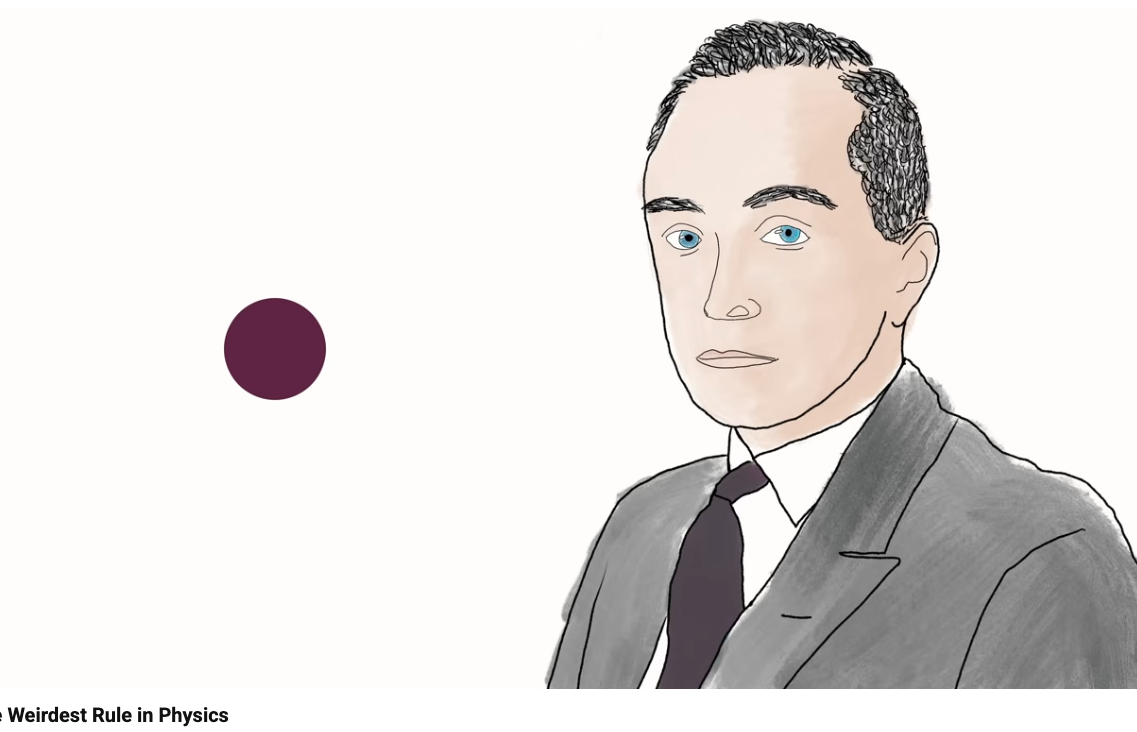
\includegraphics[width=0.7\textwidth]{born_rule.png}
        }
    \end{center}
\end{frame}

%----------------------------------------------------------------------
\begin{frame}{Claim}

\begin{block}{}
When Einstein proposed the light-quantum hypothesis in 1905 to explain
the photoelectric effect, he was doing
\textbf{machine learning} and \textbf{statistical inference}.
\end{block}

\bigskip
\begin{enumerate}
  \item \textbf{Theory} (1905): Einstein proposes a manifold of statistical models
    (an ``hypothesis class'')
  \item \textbf{Data} (1887--1916): experimenters collect data
  \item \textbf{Estimation} (1916): Millikan runs Einstein's regression and
    recovers Planck's constant to 0.5\%
\end{enumerate}

\end{frame}

%----------------------------------------------------------------------
\begin{frame}{The Photoelectric Effect and Feature Engineering}

The phenomenon (Hertz, 1887): shine light on a metal; electrons are ejected.
Apply a stopping potential $V_0$ to halt the fastest electrons.

\medskip
Lenard (1902) ran an ablation experiment---measured $V_0$ as a function of
both frequency $\nu$ and intensity $I$:

\medskip
\begin{center}
\begin{tabular}{lcc}
\toprule
Feature & Effect on $V_0$ & Importance \\
\midrule
Frequency $\nu$ & Strong $\uparrow$ & \textbf{High} \\
Intensity $I$  & None             & \textbf{Zero} \\
\bottomrule
\end{tabular}
\end{center}

\medskip
Classical wave theory predicted the opposite: $V_0$ should rise with $I$
and be independent of $\nu$.

\medskip
\textbf{ML translation:} feature-importance analysis eliminates $I$;
selects $\nu$ as sole relevant input.

\end{frame}

%----------------------------------------------------------------------
\begin{frame}{Einstein's Model and Inductive Bias}

A light quantum carries energy $E = h\nu$.
A single quantum is absorbed by a single electron.
Energy conservation gives:
\[
  \boxed{V_0 = \frac{h}{e}\,\nu - \frac{W}{e}}
\]

\begin{itemize}
  \item Slope $= h/e$ is \textbf{universal} across all metals
  \item Proposed before reliable $V_0$-vs-$\nu$ measurements existed
\end{itemize}

\medskip
The quantum hypothesis restricts the hypothesis class from \emph{all
functions} of $(\nu, I, \lambda, \ldots)$ to an affine function in
$\nu$ alone with a universal slope.

\medskip
\begin{center}
\begin{tabular}{lll}
\toprule
Hypothesis class & Dimension & Data needed \\
\midrule
All measurable functions of $(\nu, I, \ldots)$ & Infinite & $\gg 10^6$ \\
Affine in $\nu$ alone (Einstein) & 2 & $\sim 5$ \\
\bottomrule
\end{tabular}
\end{center}

\end{frame}

%----------------------------------------------------------------------
\begin{frame}{The Regression Problem}

Adding noise and a nuisance parameter:
\[
  V_{0i} = \underbrace{\alpha}_{\text{intercept}} +
            \underbrace{\beta}_{h/e}\,\nu_i +
            \underbrace{\varepsilon_i}_{\text{noise}},
  \qquad
  \alpha = -\frac{W}{e} + \underbrace{v_c}_{\text{contact EMF}}
\]

\medskip
\begin{itemize}
  \item \textbf{Training data:} $\{(\nu_i, V_{0i})\}$
  \item \textbf{Task:} estimate $\beta = h/e$ $\Rightarrow$ Planck's $h$
  \item \textbf{Loss:} squared error (OLS $=$ MLE under Gaussian errors)
  \item \textbf{Nuisance:} $v_c$ can be as large as 3\,V; shifts intercept
    but \textbf{does not bias slope} if constant within a run
\end{itemize}

\medskip
Computing the regression is trivial once you have data.
The 29-year gap between Einstein and Millikan is a data engineering problem,
not a statistical one.

\end{frame}

%----------------------------------------------------------------------
\begin{frame}{29 Years of Collecting Data (1887--1916)}

\begin{center}
\small
\begin{tabular}{p{3.2cm}cp{3.5cm}p{4.3cm}}
\toprule
Experimenter & Year & Data quality & Problem \\
\midrule
Hertz / Hallwachs & 1887--88 & Qualitative only & No labeled $(\nu,V_0)$ pairs \\
Lenard            & 1902     & Qualitative       & No reliable numerical $V_0$ \\
Hughes            & 1912     & 3 UV lines        & Contact EMF uncontrolled; 65\% scatter in $h$ \\
Richardson \& Compton & 1912 & 8 metals          & Same problems; 60\% scatter \\
\midrule
\textbf{Millikan} & \textbf{1916} &
  \textbf{Clean surfaces, wide $\Delta\nu$, controlled $v_c$} &
  \textbf{$h$ to 0.5\%} \\
\bottomrule
\end{tabular}
\end{center}

\end{frame}

%----------------------------------------------------------------------
\begin{frame}{Millikan's Experimental Design and the Cram\'er--Rao Bound}

Key data-quality innovations (``a machine shop in vacuo''):
\begin{itemize}
  \item \textbf{Fresh surfaces:} electromagnetic knife shaved alkali metal
    in vacuum---no oxidation, no work-function contamination
  \item \textbf{Spectrally pure lines:} mercury arc with filters to exclude
    UV companions
  \item \textbf{Wide frequency range:} 5461\,\AA\ to 2535\,\AA\
    ($\Delta\nu = 6.3\times10^{14}$\,Hz, a factor of two)
  \item \textbf{Controlled nuisance:} Kelvin double-balance measured $v_c$;
    stable to $\pm 0.01$\,V over 9 hours
\end{itemize}

\medskip
Cram\'er--Rao bound:
\[
  \mathrm{SE}(\hat\beta) = \frac{\sigma}{\sqrt{S_{\nu\nu}}},
  \quad S_{\nu\nu} = \sum_i(\nu_i - \bar\nu)^2
\]

\begin{center}
\small
\begin{tabular}{p{5.0cm}rrr}
\toprule
Dataset & $n$ & $S_{\nu\nu}$ ($10^{28}$ Hz$^2$) & SE($\hat\beta$) ($10^{-18}$\,V$\cdot$s) \\
\midrule
Restricted range (like Hughes) & 3 & 1.96  & 10.0 \\
Millikan full 6-pt             & 6 & 28.14 &  2.6 \\
\bottomrule
\end{tabular}
\end{center}

\end{frame}

%----------------------------------------------------------------------
\begin{frame}{Millikan's Data and OLS Result}

\begin{columns}[T]
\begin{column}{0.48\textwidth}
\begin{center}
\begin{tabular}{rrcc}
\toprule
$\lambda$ (\AA) & $\nu$ ($10^{14}$\,Hz)
  & $V_0^{\mathrm{Na}}$ & $V_0^{\mathrm{Li}}$ \\
\midrule
5461.0 &  5.490 & 0.454 & ---   \\
4339.4 &  6.908 & 1.039 & 0.499 \\
4046.8 &  7.409 & 1.246 & 0.706 \\
3650.2 &  8.213 & 1.578 & 1.037 \\
3125.5 &  9.591 & 2.147 & 1.606 \\
2534.7 & 11.827 & 3.030 & 2.529 \\
\bottomrule
\end{tabular}
\end{center}
\end{column}
\begin{column}{0.48\textwidth}
OLS on sodium (5 points):
\[
  \hat\beta = \frac{S_{\nu V}}{S_{\nu\nu}}
            = 4.129\times10^{-15}\,\text{V$\cdot$s}
\]

\begin{center}
\begin{tabular}{lr}
\toprule
$R^2$ & $\approx 0.99999$ \\
SE$(\hat\beta)$ & $4.6\times10^{-18}$\,V$\cdot$s \\
Implied $h$ & $6.573\times10^{-34}$\,J$\cdot$s \\
Error vs.\ NIST & $-0.80\%$ \\
\bottomrule
\end{tabular}
\end{center}

\medskip
$h$ to \textbf{0.5\%} from \textbf{5 data points}.
\end{column}
\end{columns}

\end{frame}

%----------------------------------------------------------------------
\begin{frame}{Universality: Zero-Shot Transfer Across Metals}

The quantum hypothesis predicts $\beta = h/e$ is the same for
\emph{all} metals.

\medskip
Separate regressions:
\begin{align*}
  \hat\beta_{\mathrm{Na}} &= 4.129\times10^{-15}\;\text{V$\cdot$s} \\
  \hat\beta_{\mathrm{Li}} &= 4.137\times10^{-15}\;\text{V$\cdot$s} \\
  \text{difference} &= 0.19\%
\end{align*}

Wald test of $H_0\colon \beta_{\mathrm{Na}} = \beta_{\mathrm{Li}}$:\quad
$z \approx 0.87$ ($\ll 1.96$). Cannot reject universality.

\medskip
In ML language:
\begin{itemize}
  \item \textbf{Pre-training:} fit slope on sodium
  \item \textbf{Zero-shot transfer:} apply slope to lithium
  \item \textbf{Fine-tuning:} only the intercept (work function)
  \item \textbf{Transfer error:} 0.2\%
\end{itemize}

\end{frame}

%----------------------------------------------------------------------
\begin{frame}{Historical Estimates of Planck's Constant}

\begin{center}
\begin{tabular}{p{4.4cm}rcr}
\toprule
Authors & Year & $h$ ($10^{-27}$\,erg$\cdot$s) & Error \\
\midrule
Hughes              & 1912 & 3.55--5.85 & $-12$ to $-46\%$ \\
Richardson \& Compton & 1912 & 3.5--5.8 & $-12$ to $-47\%$ \\
Planck (black body) & 1913 & 6.415     & $-3.2\%$         \\
\midrule
Millikan (Na, 5-pt) & 1916 & 6.573     & $-0.80\%$        \\
Millikan (Li)       & 1916 & 6.584     & $-0.64\%$        \\
\textbf{Millikan mean} & \textbf{1916} & \textbf{6.579} & $\mathbf{-0.72\%}$ \\
\midrule
Modern NIST 2022    & 2022 & 6.6261    & 0                \\
\bottomrule
\end{tabular}
\end{center}

\medskip
Pre-Millikan estimates: biased downward 10--47\%.

Three sources: stray UV, narrow $\Delta\nu$, uncontrolled $v_c$.

Millikan eliminated all three.

\end{frame}

%----------------------------------------------------------------------
\begin{frame}{Millikan's Doubts}

Millikan confirmed Einstein's equation to 0.5\%. Then wrote:

\bigskip
\begin{quote}
``Despite then the apparently complete success of the Einstein equation,
the physical theory of which it was designed to be the symbolic expression
is found \textbf{so untenable} that Einstein himself, I believe, no longer
holds to it.''
\end{quote}
\hfill Millikan (1916), p.\ 388

\bigskip
He had hoped the experiment would \textbf{refute} the equation.

\medskip
\begin{itemize}
  \item Confirming a regression equation says little about the structure that generated it
  \item Compton scattering (1923) finally convinced him
  \item Millikan's 1923 Nobel: ``\ldots first direct experimental proof
    \ldots of the complete validity of the Einstein equation''
\end{itemize}

\end{frame}

%----------------------------------------------------------------------
\begin{frame}{ML-to-Physics Dictionary}

\begin{center}
\small
\begin{tabular}{p{5.0cm}p{4.8cm}p{2.6cm}}
\toprule
\textbf{Scientific step} & \textbf{ML name} & \textbf{Who} \\
\midrule
Propose $E = h\nu$; derive $V_0 = (h/e)\nu - W/e$
  & Inductive bias + hypothesis class & Einstein (1905) \\
$V_0$ depends on $\nu$ not $I$
  & Feature engineering & Lenard (1902) \\
Measure $(\nu_i, V_{0i})$ pairs
  & Labeled training data & Millikan (1916) \\
Control contact EMF $v_c$
  & Nuisance-variable identification & Millikan (1916) \\
Min.\ $\sum(V_{0i} - \hat V_{0i})^2$
  & MSE training (OLS/MLE) & Millikan (1916) \\
$|\hat\beta - h/e| < 1\%$
  & Test accuracy & Millikan (1916) \\
Na and Li give same $\hat\beta$
  & Zero-shot transfer learning & Millikan (1916) \\
\bottomrule
\end{tabular}
\end{center}

\end{frame}

%----------------------------------------------------------------------
\begin{frame}{Einstein vs.\ a Deep Neural Network}

\begin{center}
\small
\begin{tabular}{p{2.5cm}rp{2.7cm}p{2.8cm}p{3.5cm}}
\toprule
Epoch & $n$ & Einstein model & DNN (VC $\approx$ 5700) & DNN outcome \\
\midrule
Millikan 1916 & 5  & Sufficient$^*$ & Insuf.\ ($\times 1140$) & Interpolates; no inference \\
Modern era    & $\sim 5000$ & Sufficient & Sufficient & Recovers line; cannot identify $h/e$ \\
\bottomrule
\multicolumn{5}{p{13cm}}{\small $^*$Functional form from theory; two free parameters remain.}
\end{tabular}
\end{center}

\medskip
A three-layer DNN (16 neurons/layer): $p \approx 593$ parameters,
VC dim $\approx 5700$. Reliable 1\% generalisation requires
$n \gtrsim 5700$.

\medskip
Einstein's theory made five training points sufficient---not more data,
not a better algorithm.

\medskip
DNNs win for problems without a known parametric family (images, proteins,
language). The photoelectric problem sits at the opposite extreme.

\end{frame}

%----------------------------------------------------------------------
\begin{frame}{Unintended Consequence: Born's Rule}

Einstein's quantum hypothesis required $|E|^2 \propto$ photon density.
The classical wave intensity $|E|^2$ becomes a probability density.
Einstein called this the \emph{Gespensterfeld} (ghost field).

\medskip
Max Born (1926) formalised the same logic for the Schr\"odinger wave function:
\[
  \boxed{|\psi|^2 = \text{probability density}}
\]

\medskip
Three Nobel Prizes:
\begin{itemize}
  \item 1921: Einstein---for the equation that made the measurement possible
  \item 1923: Millikan---for the measurement that confirmed it
  \item 1954: Born---for the probabilistic interpretation the equation made
    \emph{inevitable}
\end{itemize}

\medskip
Einstein spent the rest of his life rejecting Born's rule.
He won the Nobel for a paper whose logic seeded the interpretation he most
opposed.

\end{frame}

%----------------------------------------------------------------------
\begin{frame}{Summary}

\begin{block}{The Thesis}
Einstein was doing machine learning in 1905---but the step no ML system
has automated is \textbf{specifying the hypothesis class}.
\end{block}

\bigskip
\begin{enumerate}
  \item \textbf{Theoretical priors guide design.} $E=h\nu$ fixes the
    functional form; 5 training points suffice for 0.1\% precision.
  \item \textbf{Data quality is the binding constraint.} The regression
    is trivial; assembling good data took 29 years.
  \item \textbf{Confirming an equation $\neq$ endorsing the model.}
    Millikan confirmed the slope to 0.5\% while rejecting the
    light-quantum interpretation.
\end{enumerate}

\bigskip
A data-driven system given only $(\nu_i, V_{0i})$ pairs can recover
$\hat\beta = 4.129\times10^{-15}$\,V$\cdot$s but cannot know it is $h/e$.
\textbf{Physical meaning requires physical theory.}

\end{frame}

%----------------------------------------------------------------------
\begin{frame}{References}

\small
\begin{itemize}
  \item Einstein, A.\ (1905). ``\"Uber einen die Erzeugung und Verwandlung
    des Lichtes betreffenden heuristischen Gesichtspunkt.''
    \textit{Ann.\ Phys.}, 17, 132--148.
  \item Lenard, P.\ (1902). ``\"Uber die lichtelektrische Wirkung.''
    \textit{Ann.\ Phys.}, 8, 149--198.
  \item Millikan, R.\,A.\ (1916). ``A Direct Photoelectric Determination
    of Planck's $h$.'' \textit{Phys.\ Rev.}, 7(3), 355--388.
  \item Born, M.\ (1926). ``Zur Quantenmechanik der
    Sto{\ss}vorg\"ange.'' \textit{Z.\ Phys.}, 37, 863--867.
  \item Hughes, A.\,L.\ (1913). ``On the Emission Velocities of
    Photo-Electrons.'' \textit{Phil.\ Trans.\ R.\ Soc.\ A}, 212, 205--226.
  \item Richardson, O.\,W.\ \& Compton, K.\,T.\ (1912). ``The
    Photoelectric Effect.'' \textit{Phil.\ Mag.}, 24, 575--594.
  \item Udrescu, S.\,M.\ \& Tegmark, M.\ (2020). ``AI Feynman.''
    \textit{Sci.\ Adv.}, 6, eaay2631.
  \item Vapnik, V.\ (1998). \textit{Statistical Learning Theory}.
    Wiley.
\end{itemize}

\end{frame}

%----------------------------------------------------------------------
\end{document}
